\begin{figure}[H]
\centering
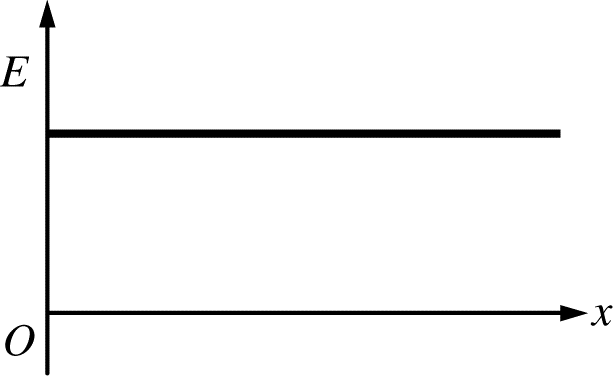
\includegraphics[scale=0.25]{images/img-009-029.png}
\end{figure}

% Multiple Choice Question 16
\begin{questions}\setcounter{question}{15}\question
The graph above shows the electric field $E$ as a function of $x$, where $x$ is the distance from a given charge arrangement in an $x y z$-coordinate system. Which of the following could be the arrangement?

\begin{choices}
\choice A positive point charge at $x=0$
\choice Positive charges uniformly distributed inside a sphere with $x=0$ on the sphere's surface
\choice Positive charges uniformly distributed on the surface of a sphere with $x=0$ on the sphere's surface
\choice Positive charges uniformly distributed along the $y$-axis
\choice Positive charges uniformly distributed over the $y z$-plane
\end{choices}\end{questions}

